% =====================================================================================
% PLANTILLA ACADÉMICA APA 7 (SÉPTIMA EDICIÓN) — CONFIGURACIÓN NATIVA EN LaTeX
% Motor recomendado: pdfLaTeX + Biber (Overleaf detecta Biber automáticamente
% al encontrar \addbibresource). Compilar 2-3 veces para resolver TOC/Bibliografía.
% =====================================================================================
\documentclass[12pt,letterpaper]{article}

% --------------------------- ARCHIVO .bib EMBEBIDO (DEMO) ---------------------------
\usepackage{filecontents} 

\begin{filecontents*}{referencias.bib}
@article{autor2024ejemplo,
  author       = {Apellido, Nombre A.},
  title        = {Título completo del artículo de ejemplo en formato sentencia},
  journaltitle = {Nombre de la Revista Científica},
  year         = {2024},
  volume       = {12},
  number       = {3},
  pages        = {45--60},
  doi          = {10.1000/ejemplo.doi}
}
@book{autor2023libro,
  author    = {Apellido, Nombre B.},
  title     = {Título del libro de ejemplo},
  year      = {2023},
  publisher = {Editorial Ejemplo},
  location  = {Ciudad, País}
}
\end{filecontents*}

% --------------------------------- CODIFICACIÓN --------------------------------------
\usepackage[utf8]{inputenc}
\usepackage[T1]{fontenc}
\usepackage[spanish]{babel} 

% ------------------------------ MÁRGENES (1 PULGADA) ---------------------------------
\usepackage[letterpaper, margin=1in]{geometry}

% ------------------------------ INTERLINEADO DOBLE ------------------------------------
\usepackage{setspace}
\setstretch{2.0}

% --------------------------------- TIPOGRAFÍA -----------------------------------------
\usepackage{times} 

% --------------------------- SANGRÍA Y ALINEACIÓN DE PÁRRAFOS -------------------------
\usepackage{indentfirst}         
\usepackage{ragged2e}
\RaggedRight                        
\setlength{\parindent}{0.5in}       
\setlength{\parskip}{0pt}           

% ------------------------------ FIGURAS Y TABLAS (FORMATO APA) ------------------------
\usepackage{graphicx}
\usepackage{booktabs}   
\usepackage{caption}
\usepackage{placeins} % Evita que las figuras "floten" más allá de su sección

\captionsetup[figure]{
  font={bf}, labelfont={bf}, textfont={it},
  justification=centering, singlelinecheck=false,
  position=top, name=Figura, labelsep=newline
}
\captionsetup[table]{
  font={bf}, labelfont={bf}, textfont={it},
  justification=centering, singlelinecheck=false,
  position=top, name=Tabla, labelsep=newline
}

% Comando para la "Nota." descriptiva al pie de figuras/tablas (alineada a la izquierda)
\newcommand{\aparnote}[1]{\par\vspace{4pt}\noindent\RaggedRight\textit{Nota.} #1\par}

% ------------------------- ENCABEZADO Y PAGINADO MODIFICADO ---------------------------
\usepackage{fancyhdr}
\setlength{\headheight}{28pt} % Altura suficiente para los logos pequeños
\pagestyle{fancy}
\fancyhf{}

% Logo de la Universidad en la esquina superior IZQUIERDA
\fancyhead[L]{
\includegraphics[height=0.8cm]{Logos/LogoUniversidad.png}}

% Número de página y Logo de la Carrera en la esquina superior DERECHA
\fancyhead[R]{%
  \thepage \hspace{0.3cm}% Puedes cambiar el orden si prefieres el logo antes que el número
  
\includegraphics[height=0.8cm]{Logos/LogoCarrera.png}%
}
\renewcommand{\headrulewidth}{0pt}

% --------------------------- JERARQUÍA DE 5 NIVELES DE TÍTULO APA 7 -------------------
\usepackage{titlesec}
\setcounter{secnumdepth}{0}  
\setcounter{tocdepth}{3}     

% Nivel 1: Centrado, Negrita, Tipo Título
\titleformat{\section}{\centering\bfseries}{}{0pt}{}
\titlespacing*{\section}{0pt}{0pt}{0pt}

% Nivel 2: Alineado a la izquierda, Negrita Tipo Título
\titleformat{\subsection}{\flushleft\bfseries}{}{0pt}{}
\titlespacing*{\subsection}{0pt}{0pt}{0pt}

% Nivel 3: Alineado a la izquierda, Negrita Cursiva, Tipo Título
\titleformat{\subsubsection}{\flushleft\bfseries\itshape}{}{0pt}{}
\titlespacing*{\subsubsection}{0pt}{0pt}{0pt}

% Nivel 4: Sangrado, Negrita, Tipo Título, con punto final, el texto continúa en la misma línea
\titleformat{\paragraph}[runin]{\bfseries}{}{0pt}{}[.]
\titlespacing*{\paragraph}{\parindent}{0pt}{1em}

% Nivel 5: Sangrado, Negrita Cursiva, Tipo Título, con punto final, texto continúa en la misma línea
\titleformat{\subparagraph}[runin]{\bfseries\itshape}{}{0pt}{}[.]
\titlespacing*{\subparagraph}{\parindent}{0pt}{1em}

% --------------------------------- LOREM IPSUM (RELLENO) ------------------------------
\usepackage{lipsum}

% --------------------------------- BIBLIOGRAFÍA APA 7 ----------------------------------
\usepackage{csquotes}
\usepackage[backend=biber, style=apa]{biblatex}
\addbibresource{referencias.bib} 

% --------------------------------- HIPERVÍNCULOS (OPCIONAL, SIN COLOR) -----------------
\usepackage[hidelinks]{hyperref}
\hypersetup{
  pdftitle={Título del Trabajo}, 
  pdfauthor={Nombre del Autor}  
}

% =====================================================================================
\begin{document}
% =========================== PORTADA ESTUDIANTIL MODIFICADA ===========================
\thispagestyle{empty} % Esto asegura que la portada no tenga el encabezado con logos ni número de página

% Encabezado superior con bloques de alineación invisibles para placeholders de logos en portada
\noindent
\begin{minipage}{0.5\textwidth}
    \flushleft
    
\includegraphics[height=3cm]{Logos/LogoUniversidad.png}
\end{minipage}%
\begin{minipage}{0.5\textwidth}
    \flushright
    
\includegraphics[height=3cm]{Logos/LogoCarrera.png}
\end{minipage}

\begin{center}
\vspace*{1.5in}

\textbf{AE10. Avances de proyecto}\\
\vspace{\baselineskip} 

Brandon Chavarría Ángeles\\
Kenneth Morán Gómez\\
Emmanuel Islas Lozada\\
José Enrique Sánchez Romero\\
Universidad Politécnica de Pachuca\\
Mantenimiento de Software\\
Alicia Ortíz Montes\\
17 de Agosto de 2026

\end{center}
\newpage

% ============================== ÍNDICES AUTOMATIZADOS =================================
\tableofcontents
\newpage
\listoffigures
\newpage
\listoftables
\newpage

% ============================ CUERPO DEL DOCUMENTO =====================================

\section{Introducción}
El presente documento reporta el avance real del proyecto de mantenimiento de software del sistema Yoliztli, contrastado contra la planeación SCRUM establecida por el equipo. El objetivo de este entregable (AE10) es documentar, con evidencia verificable, el estado del backlog al 17 de agosto de 2026, la herramienta de seguimiento utilizada (GitHub Projects) y la gráfica de quemado (\textit{burndown chart}) correspondiente al sprint en curso.

\subsection{Antecedentes del Estudio}
La planeación original del equipo estableció un backlog total de 20 puntos de historia (SP), distribuidos en dos sprints de dos semanas cada uno: Sprint 1 (Infraestructura y Datos, 13 SP) y Sprint 2 (Lógica y Calidad, 7 SP). Dicha planeación derivó del diagnóstico inicial documentado mediante SonarQube y de las pruebas funcionales de caja negra aplicadas al sistema.

\subsubsection{Alcance de este Reporte}
Este reporte cubre únicamente el corte de avance al cierre del Sprint 1, sin proyectar resultados de Sprint 2, que aún no ha iniciado formalmente.

\newpage
\section{Metodología}
El seguimiento del proyecto se realizó mediante \textbf{GitHub Projects}, vinculado directamente al repositorio del código fuente. Se configuraron los siguientes elementos:

\begin{itemize}
\item Un tablero (\textit{board}) con un \textit{issue} por cada Solicitud de Modificación (MR-001 a MR-005), replicando la tabla de PR/MR de la planeación original.
\item Campos personalizados de \textbf{Prioridad} (Crítica, Alta, Media, Baja) y \textbf{Sprint} (Sprint 1, Sprint 2), para agrupar y filtrar el backlog.
\item Un flujo de trabajo (\textit{workflow}) que vincula cada \textit{Pull Request} (PR) a su \textit{issue} correspondiente mediante la palabra clave \texttt{Closes~\#N}, de forma que el cierre del \textit{issue} solo ocurre cuando el código respectivo ha sido fusionado a la rama principal.
\end{itemize}

Esta metodología distingue explícitamente dos niveles de avance: (1) \textit{trabajo codificado}, es decir, funcionalidad ya programada pero pendiente de fusión, y (2) \textit{trabajo verificado}, es decir, funcionalidad respaldada por un \textit{issue} cerrado automáticamente vía PR fusionado. Esta distinción es la base de la gráfica de quemado presentada en la sección de Resultados.

\begin{figure}[h]
\centering
\caption{Tablero de GitHub Projects del Proyecto Yoliztli}
\label{fig:github-board}
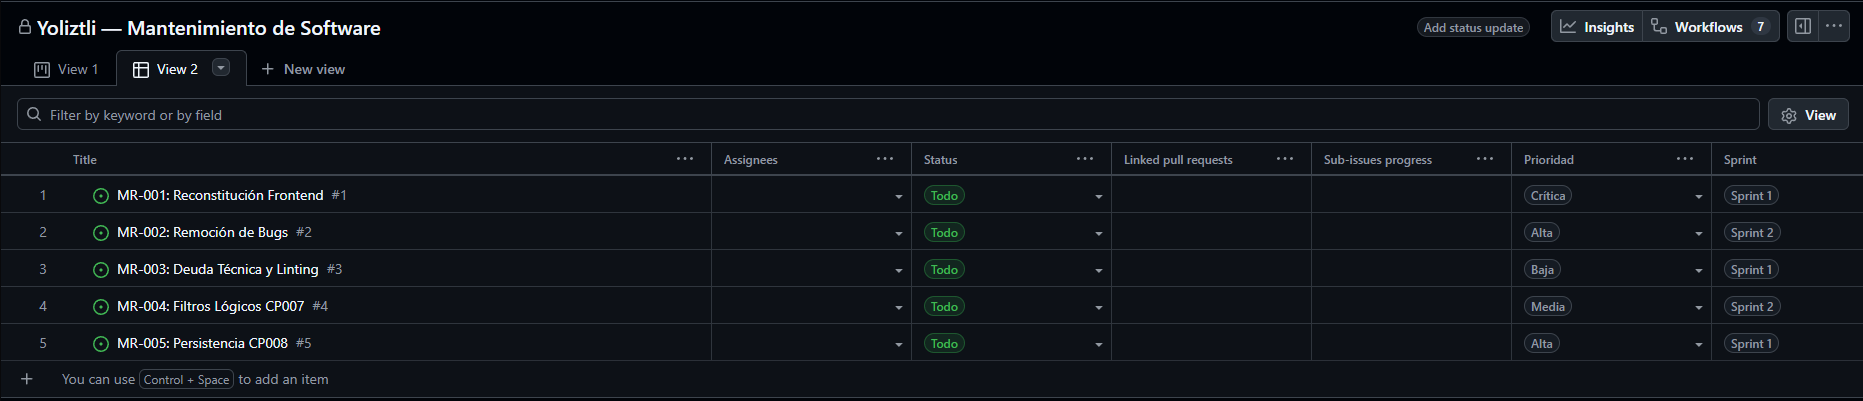
\includegraphics[width=0.95\linewidth]{img/github_board.png}
\aparnote{Vista de tabla del Project mostrando los cinco \textit{issues} (MR-001 a MR-005) con sus campos de Prioridad y Sprint asignados. Captura propia, 17 de agosto de 2026.}
\end{figure}
\FloatBarrier

\newpage
\section{Resultados}

\subsection{Contraste entre Planeación y Avance Real}
La Tabla~\ref{tab:avance} contrasta el backlog planeado por sprint contra el estado real observado en el tablero de GitHub Projects al momento del corte.

\begin{table}[h]
\centering
\caption{Avance real contrastado con la planeación por sprint}
\label{tab:avance}
\begin{singlespace}
\begin{tabular}{lccl}
\toprule
Sprint & SP Planeados & SP Codificados & Estado en GitHub \\
\midrule
Sprint 1 (Infraestructura y Datos) & 13 & 13 & PR abiertos, sin fusionar \\
Sprint 2 (Lógica y Calidad) & 7 & 0 & No iniciado \\
\bottomrule
\end{tabular}
\end{singlespace}
\aparnote{SP = Story Points. ``Codificados'' refiere a funcionalidad ya programada (vistas React reconstituidas y persistencia del progreso infantil); ninguna ha sido fusionada a \texttt{main} al corte de este reporte, por lo que el conteo verificable en GitHub es de 0 \textit{issues} cerrados. Elaboración propia.}
\end{table}

El equipo completó la programación del 100\% del alcance de Sprint 1 
(MR-001: reconstitución del frontend; MR-005: persistencia del progreso 
infantil), lo cual coloca al equipo ligeramente adelantado respecto al ritmo 
ideal de una historia por día. Sin embargo, ninguno de los 
\textit{Pull Requests} correspondientes ha sido fusionado a la rama principal 
al momento de este corte, por lo que el avance \textit{verificable} mediante 
\textit{issues} cerrados es de 0 SP.

\newpage

\subsection{Gráfica de Quemado (Burndown Chart)}
La Figura~\ref{fig:burndown} presenta la gráfica de quemado real del proyecto, distinguiendo la línea ideal planeada, el avance de trabajo codificado y el avance verificado formalmente en GitHub.

\begin{figure}[h]
\centering
\caption{Gráfica de Quemado — Estado Real al 17 de Agosto de 2026}
\label{fig:burndown}
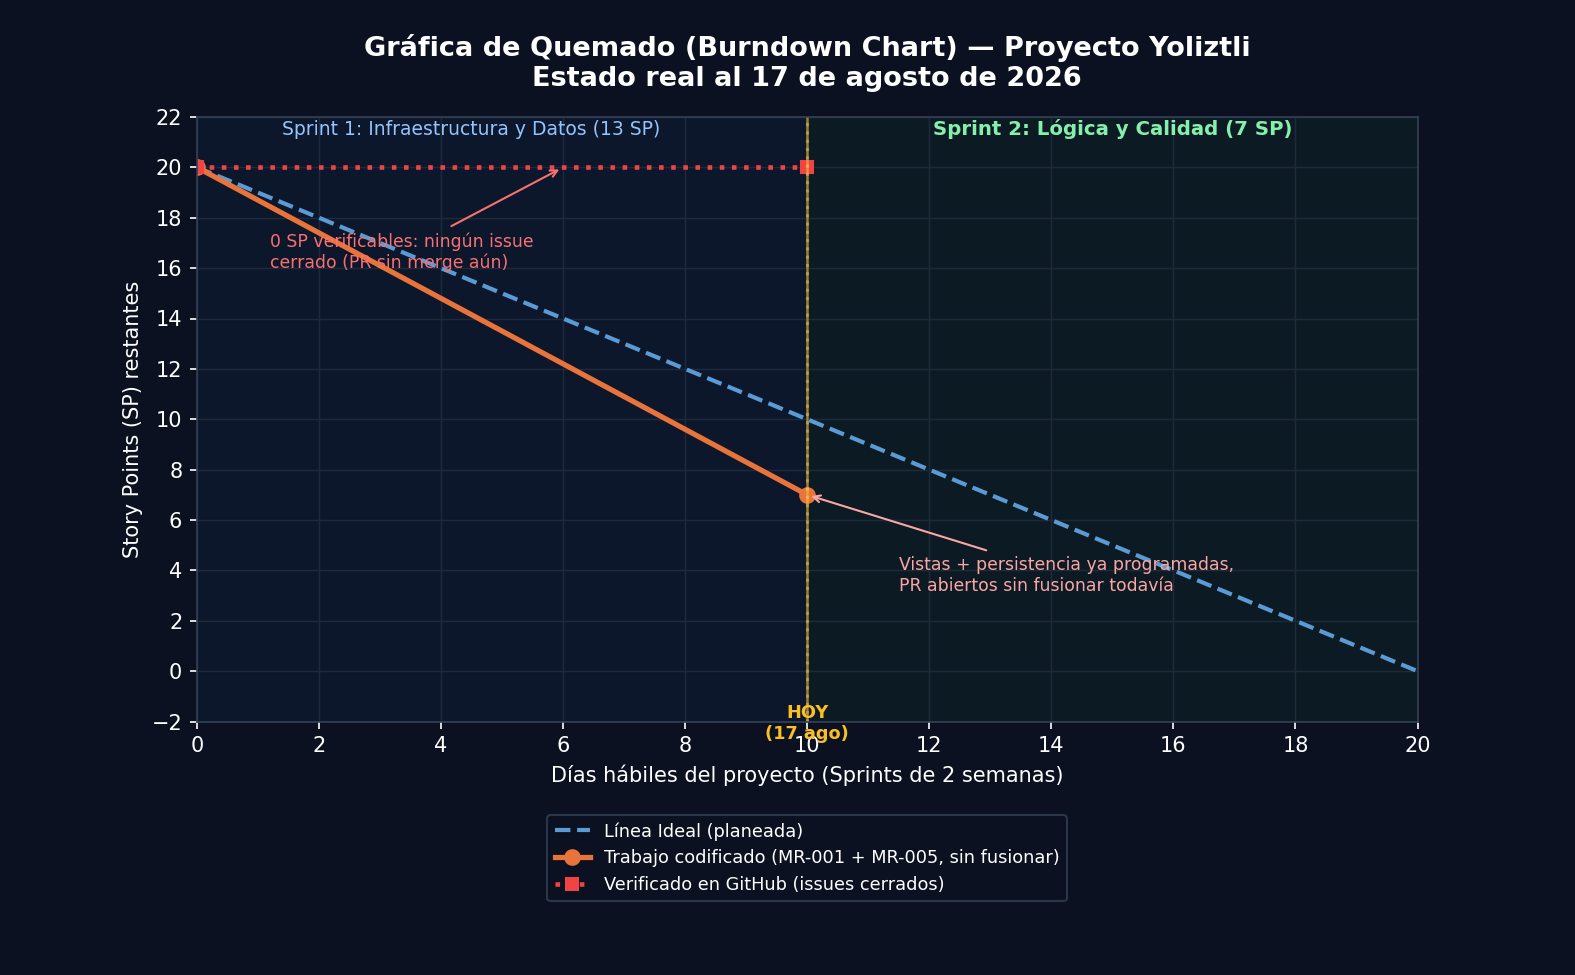
\includegraphics[width=0.95\linewidth]{img/burndown_yoliztli_real.png}
\aparnote{La línea punteada azul representa el ritmo ideal (20 SP en 20 días hábiles). La línea naranja representa el trabajo ya codificado (13 SP). La línea roja punteada representa el avance verificado mediante \textit{issues} cerrados en GitHub (0 SP), dado que los \textit{Pull Requests} de MR-001 y MR-005 permanecen abiertos. Elaboración propia.}
\end{figure}
\FloatBarrier

\newpage

\section{Discusión}
El contraste entre la línea de trabajo codificado y la línea de trabajo 
verificado evidencia una brecha de proceso más que una brecha de desarrollo: 
el equipo cumplió el alcance funcional de Sprint 1 dentro del tiempo planeado,
pero el flujo formal de cierre de \textit{issues} vía \textit{Pull Request} 
fusionado aún no se ha completado. Esta brecha es de bajo riesgo y de 
resolución inmediata: basta con fusionar los PR abiertos de MR-001 y MR-005 
incluyendo la palabra clave \texttt{Closes} en su descripción para que la 
línea verificada coincida con la línea de trabajo codificado.

Como siguiente paso, el equipo fusionará dichos \textit{Pull Requests} antes de iniciar formalmente el Sprint 2 (Lógica y Calidad: MR-002, MR-003 y MR-004), de manera que cada sprint quede cerrado con evidencia trazable de \textit{commits}, PR e \textit{issues} antes de avanzar al siguiente.

% ================================== REFERENCIAS =========================================


\end{document}